\documentclass[12pt]{article}
\usepackage{amsmath}
\usepackage{mathtools}
\usepackage{bigints}
\usepackage{parskip}
\usepackage{amssymb}
\usepackage{relsize}
\usepackage{fullpage}
% \DeclareMathSizes{12}{17.28}{9}{7} % (a)

\DeclareMathSizes{12}{17.28}{12}{12} % (a)


\usepackage{hyperref}



	\addtolength{\topmargin}{-.5in}
	\addtolength{\textheight}{1.75in}



    \newenvironment{myindentpar}[1]%
     {\begin{list}{}%
             {\setlength{\leftmargin}{#1}}%
             \item[]%
     }
     {\end{list}}

\begin{document}
\title{College Algebra: Module 6 What You Need To Know}
\date{2-26-15}
\author{}
\maketitle


\section{Solving Other Types of Equations (Section 1.6)}

- Just going to do example problems and for solving various types of equations


\section{Rectangular Coordinates: Graphing Circles and Other Relations (Section 2.1)}

\textbf{Distance Between Two Points:} 
\newline

\centerline{$d \Big((x_{1},y_{1}),(x_{2},y_{2})\Big) = \sqrt{(x_{2}-x_{1})^2+(y_{2}-y_{1})^2}$}

\textbf{Midpoint Between Two Points:} 
\newline

\centerline{$M \Big((x_{1},y_{1}),(x_{2},y_{2})\Big) =\Big(\dfrac{x_{1}+x_{2}}{2}, \dfrac{y_{1}+y_{2}}{2}\Big)$}

\textbf{Parabolas:} 

\centerline{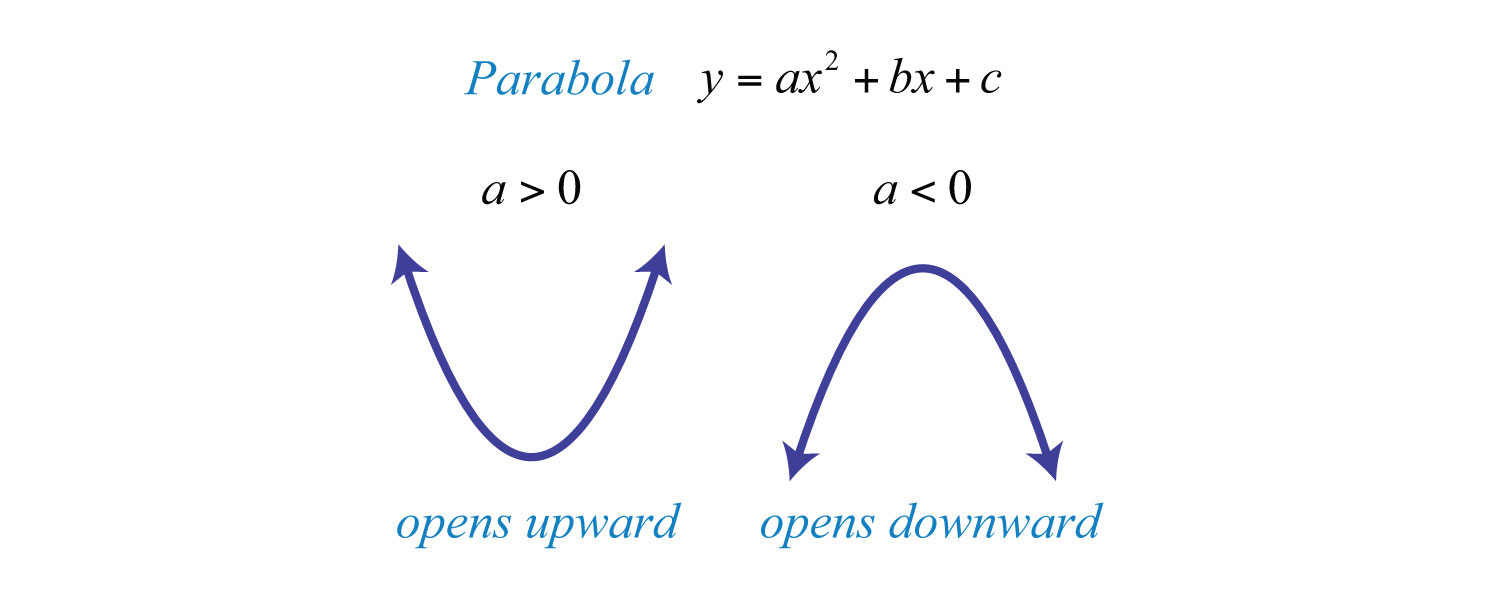
\includegraphics[scale = 0.3]{Parabola.jpg}}

\newpage

\textbf{Cubics:} 

\centerline{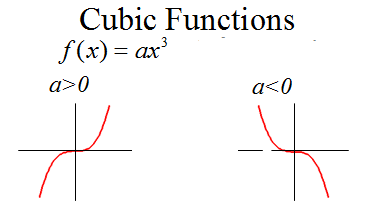
\includegraphics{Cubic.png}}

\textbf{Standard Equation for a Circle:} 
\newline

\centerline{$(x-h)^2+(y-k)^2=r^2$}
\vspace{.5cm}
\centerline{\textbf{Center:} $(h,k)$ \hspace{2cm} \textbf{Radius:} $\sqrt{r^2} = r$}

\vspace{1cm}

\textbf{Word Problem: (Multiple Rates)} A swimming pool holds $480,000$  liters of water. The pool has two drainage pipes. When the pool is completely full, the first pipe alone can empty it in $240$ minutes, and the second pipe alone can empty it in $160$ minutes. When both pipes are draining together, how long does it take them to empty the pool?

















\end{document}